\documentclass[tikz, border=2pt]{standalone}

\usepackage{helvet}
\renewcommand{\familydefault}{\sfdefault}

\usepackage[EULERGREEK]{sansmath}
\sansmath
\usetikzlibrary{arrows.meta}

\begin{document}%

\begin{tikzpicture}[line width=2pt]
\tikzset{>={Latex[width=3mm,length=4mm]}}

% grid
% \draw[help lines] (-0.5, -5) grid (13, 18);


\node[inner sep=0pt] (figa) at (1.5,13.3)
{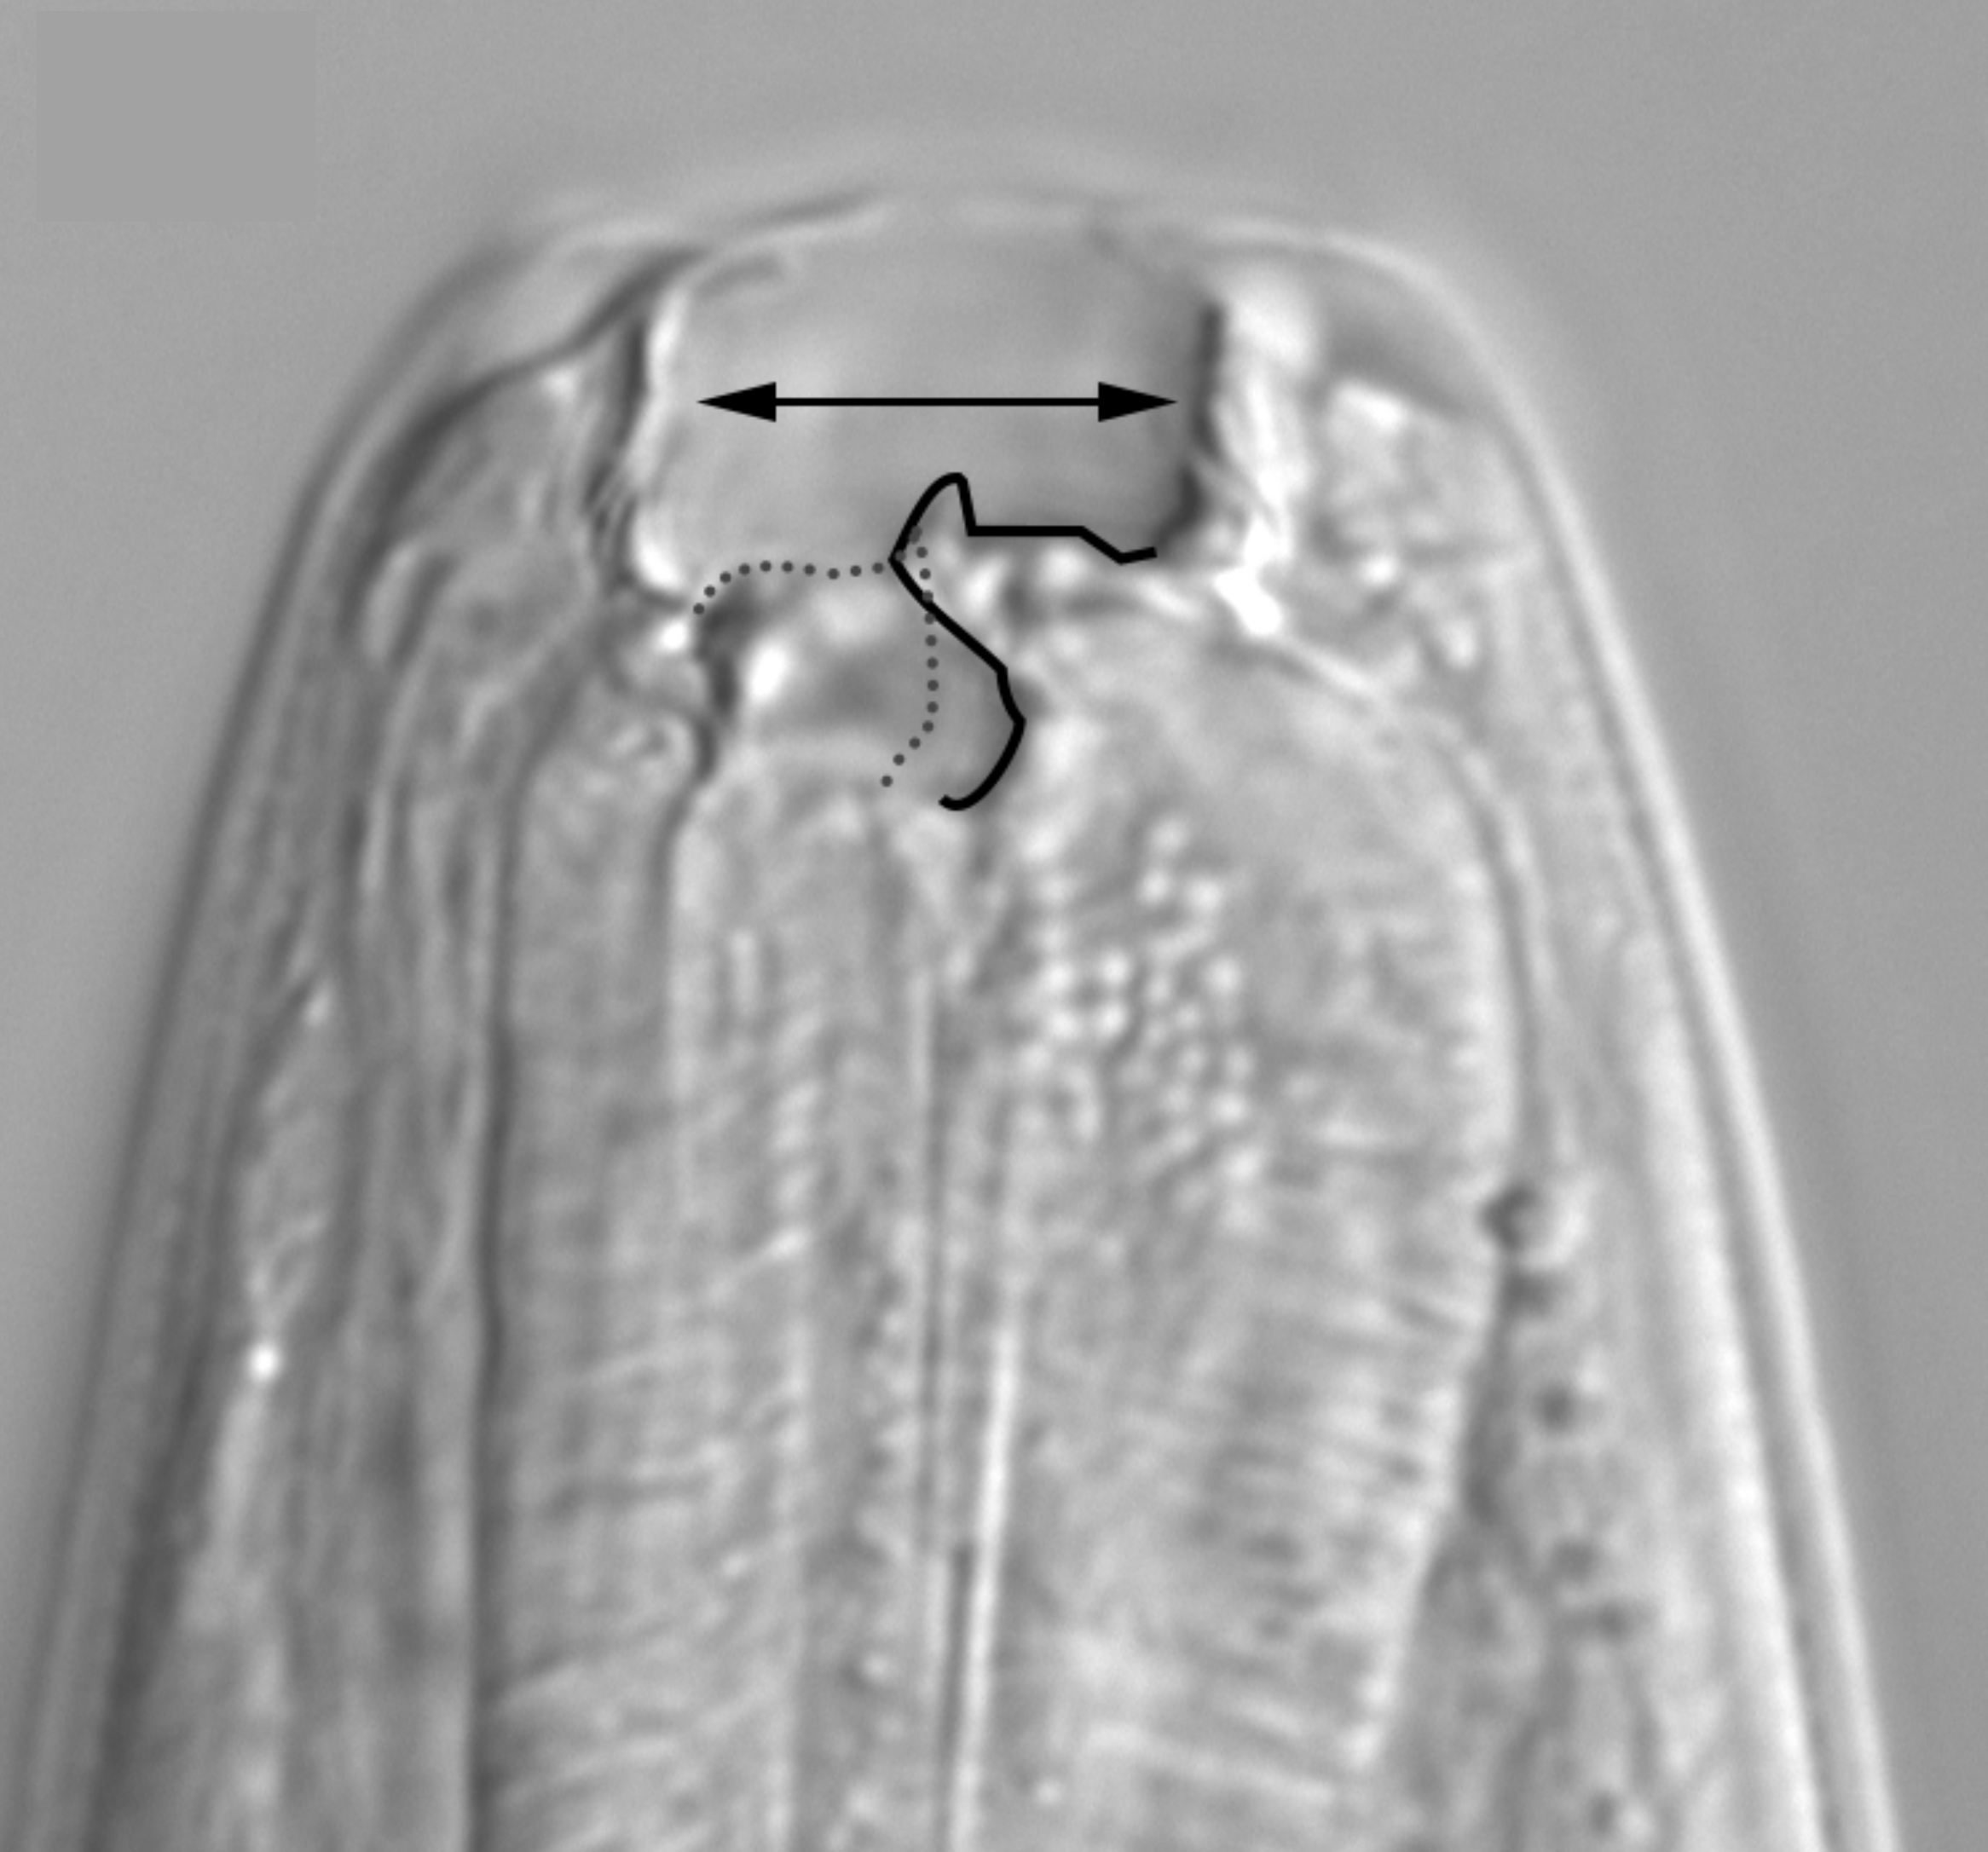
\includegraphics[width=0.15\textwidth]{eu_wol.png}};

\node[inner sep=0pt] (figa) at (3.6,13.3)
{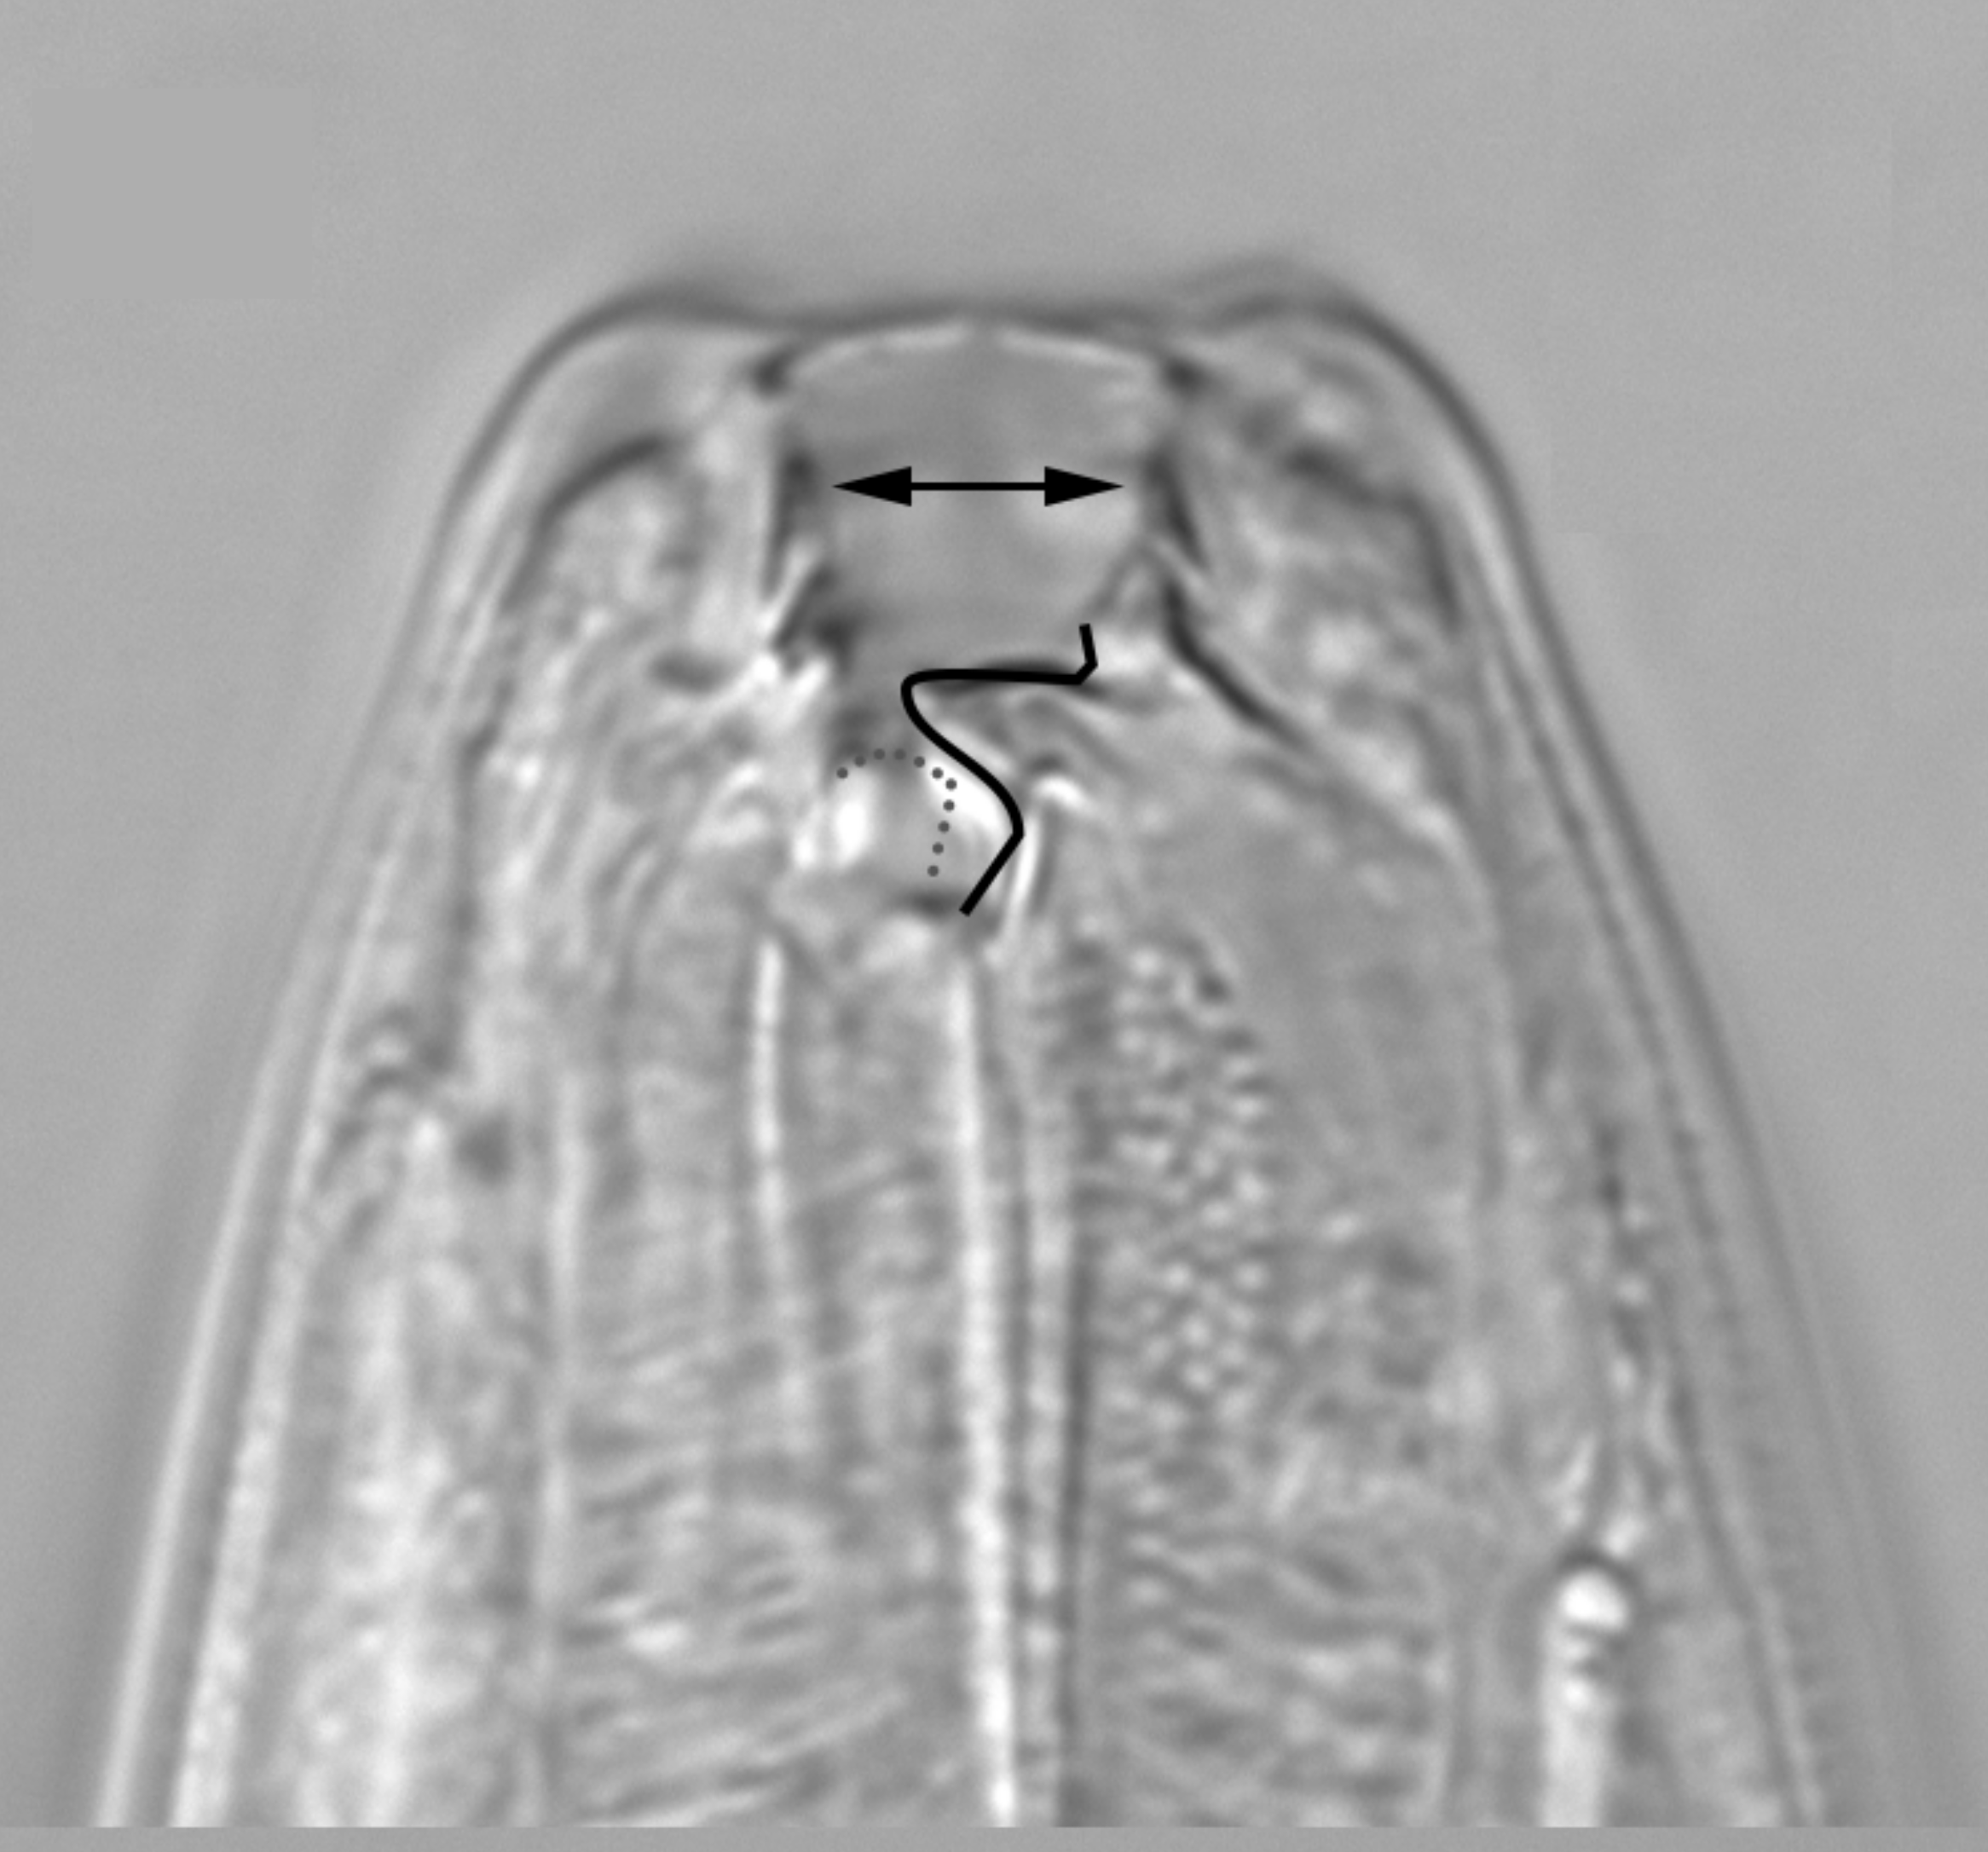
\includegraphics[width=0.15\textwidth]{st_wol.png}};

\node[rotate=0] at (1.4,12) {\footnotesize Eurystomatous};
\node[rotate=0] at (3.6, 12) {\footnotesize Stenostomatous};

  \node[inner sep=0pt] (figa) at (6,8.8)
  {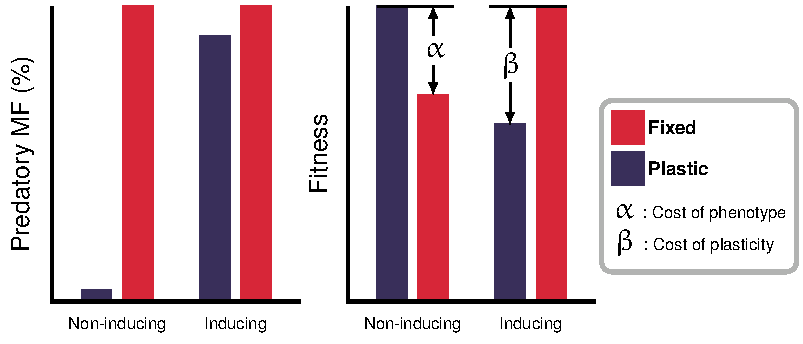
\includegraphics[width=0.9\textwidth]{figure1e.pdf}};

  \node[inner sep=0pt] (figa) at (9,13.3)
  {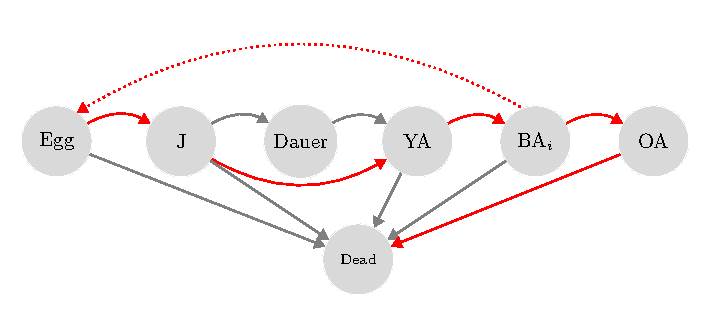
\includegraphics[width=0.7\textwidth]{markov_chain.pdf}};

  \node[inner sep=0pt] (figa) at (6.9,2.8)
  {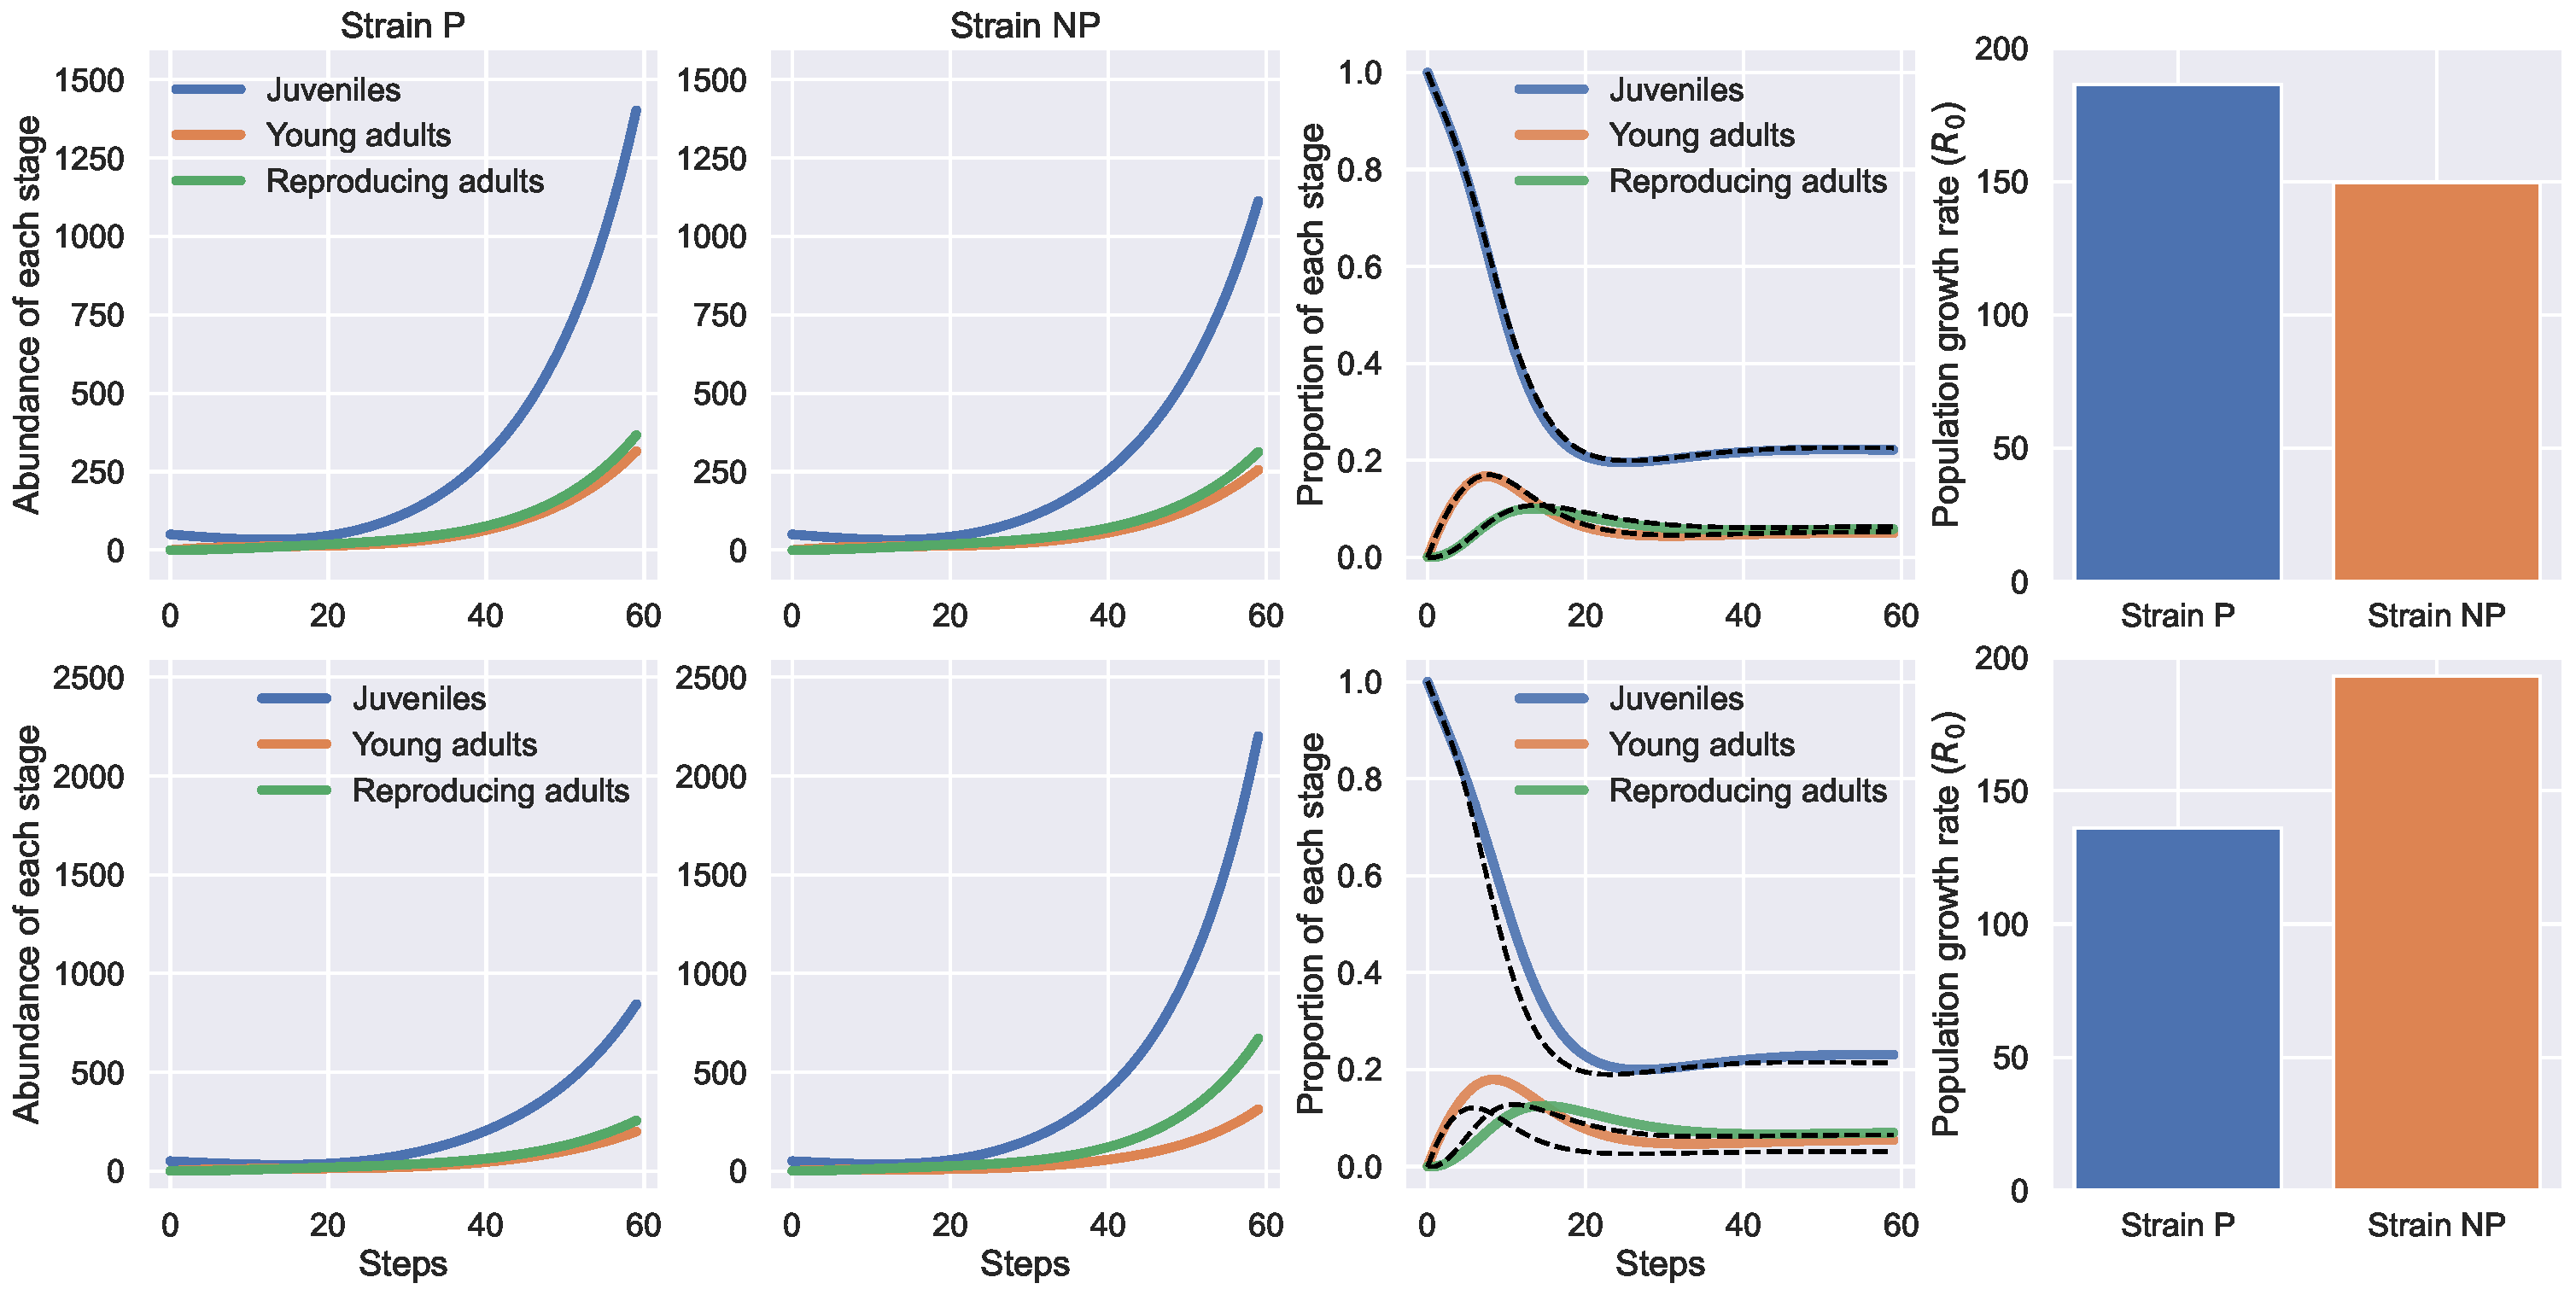
\includegraphics[width=1.1\textwidth]{PopDynamic_no_interaction.pdf}};


\node at (-0.,4.5) [draw=white, rectangle, rotate=90] (g1) {\sf \small \emph{E. coli} OP50};

\node at (-0.,1.3) [draw=white, rectangle, rotate=90] (g1) {\sf \small \emph{Novosphingobium}};



%labels
\draw (0., 14.8) node{{\Huge\sf\textbf{a}}};

\draw (5, 14.8) node{{\Huge\sf\textbf{b}}};

\draw (0., 11.5) node{{\Huge\sf\textbf{c}}};

\draw (0., 6.3) node{{\Huge\sf\textbf{d}}};


\end{tikzpicture}


\end{document}